% Bedienoberfläche
\tikzstyle{every node}=[draw=white,thin,anchor=west]
\tikzstyle{selected}=[draw=red,fill=red!30]
\tikzstyle{optional}=[dashed,fill=gray!30]


\section{Bedienoberfläche}

\subsection{Struktur Frontend}
\label{Struktur Frontend}

Als erste Ansicht der Webapplikation soll eine Deutschlandkarte mit farbigen \glspl{Kartenoverlays} geladen werden. Die farbigen \glspl{Kartenoverlays} geben hierbei Feinstaubdaten wieder.
Die Webapplikation kann von einer ausklappbaren Toolbar aus bedient werden. Von dort aus sind die verschiedenen Seiten der Webapplikation erreichbar und deren Funktionen abrufbar. 
Dabei bieten sich dem Nutzer die hier dargestellten Optionen. Erweiterte Funktionen sind in den folgenden Diagrammen grau hinterlegt.

\begin{tikzpicture}[%
grow via three points={one child at (0.5,-0.7) and
	two children at (0.5,-0.7) and (0.5,-1.4)},
edge from parent path={(\tikzparentnode.south) |- (\tikzchildnode.west)}]
\node {Toolbar}
child{ node {Aktuelle Daten (Startseite)}
	child { node {Luftqualitätsdaten}
		child { node {Feinstaub (Startseite)}}
		child { node {Luftdruck}}
		child { node {Lufttemperatur}}
		child { node {Luftfeuchtigkeit}}
		child { node [optional]{Filtertyp (Experten Modus)}}
	}
	child [missing] {}				
	child [missing] {}				
	child [missing] {}	
	child [missing] {}
	child [missing] {}
	child { node {Suchfunktion Ort}}
}
child [missing] {}				
child [missing] {}				
child [missing] {}	
child [missing] {}
child [missing] {}
child [missing] {}	
child [missing] {}											
child { node {Zeitliche Entwicklung}}
child { node {Definition von Feinstaub}}
child { node [optional]{Hauptgründe für Feinstaub in Deutschland}}
child { node [optional]{Gesundheitsrisiken von Feinstaub}}
child { node {\glspl{SmartAQnet}}}
child { node [optional]{Verlinkung zu einer Bauanleitung für einen \glspl{DIY-Sensor}}}
child { node [optional]{Hilfe Funktion}}
child { node [optional] {Spracheinstellung}
	child { node {Deutsch}}
	child { node [optional] {Englisch}}
}
child [missing] {}				
child [missing] {}
child { node [optional] {Modus}
	child { node {Normaler Modus}}
	child { node [optional]{Dark Mode}}
	child { node [optional] {Experten Modus}}
	child { node [optional] {Farbenblind Modus}}
};
\end{tikzpicture}

\subsubsection{Aktuelle Daten (Startseite)}

''Aktuelle Daten'' zeigt eine Karte von Deutschland mit der der Nutzer interagieren kann. Er kann in der Toolbar auswählen welche Luftqualitätsdaten er mit farbigen \glspl{Kartenoverlays} auf der Landkarte angezeigt haben möchte. Dabei hat er die Auswahl zwischen Daten zu Feinstaub, Lufttemperatur, Luftdruck und Luftfeuchtigkeit.
Der Nutzer kann Orte auf der Landkarte suchen. Er kann Sensoren oder Punkte auf der Landkarte auswählen und genauere Luftqualitätsdaten zu ihnen erhalten. Dies soll durch die Sidebar ermöglicht werden.
Die Sidebar ist ein funktionaler Teil der Seite Aktuelle Daten-Deutschlandkarte. Klickt der Nutzer auf einen Sensor oder einen Punkt auf der Karte öffnet sie sich automatisch.

\begin{tikzpicture}[%
grow via three points={one child at (0.5,-0.7) and
	two children at (0.5,-0.7) and (0.5,-1.4)},
edge from parent path={(\tikzparentnode.south) |- (\tikzchildnode.west)}]
\node {Sidebar}
child { node {Sensortyp}}
child { node {Messwerte}}
child { node {Diagramm}}
child { node {Suchfunktion Datum}
	child { node {Messwerte bei ausgewähltem Datum}}
}
child [missing] {}
child { node [optional] {Gesundheitsrisiken zu den Messwerten}};
\end{tikzpicture}

\subsubsection{Zeitliche Entwicklung}

In \enquote Zeitliche Entwicklung'' soll es dem Nutzer ermöglicht werden sich mit der zeitlichen Entwicklung der Luftqualität auseinanderzusetzen. Zu diesem Zweck sollen Feinstaubdaten als farbige Overlays auf einer Deutschlandkarte mit Zeitachse angezeigt werden. Der Nutzer durch das Verschieben eines Schalters auf der Zeitachse Messwerte an verschiedenen Zeitpunkten auf der Karte aufrufen.

\begin{tikzpicture}[%
grow via three points={one child at (0.5,-0.7) and
	two children at (0.5,-0.7) and (0.5,-1.4)},
edge from parent path={(\tikzparentnode.south) |- (\tikzchildnode.west)}]
\node {Zeitachse}
child { node {Schiebefunktion des Zeitpunkts}};
\end{tikzpicture}

\subsubsection{Definition von Feinstaub}
Auf dieser Seite soll eine verständliche Definition von Feinstaub wiedergegeben werden.


\subsubsection{Hauptgründe für Feinstaub in Deutschland}
Diese Seite soll die Gründe für Feinstaub in Deutschland graphisch darstellen.


\subsubsection{Gesundheitsrisiken von Feinstaub}
Die Seite ''Gesundheitsrisiken von Feinstaub'' soll dem Nutzer sachlich aufzeigen welche Gesundheitsrisiken durch Feinstaub kurzfristig und langfristig auftreten. Dabei sollen ebenfalls graphische Hilfsmittel eingesetzt werden.

\subsubsection{SmartAQnet}
An dieser Stelle soll eine kurze Beschreibung über das Projekt \glspl{SmartAQnet} informieren.Ebenso gibt es eine Verlinkung zum Projekt \glspl{SmartAQnet}.

\subsubsection{Verlinkung zu einer Bauanleitung für einen \glspl{DIY-Sensor}}
Verlinkung zu einer Bauanleitung für einen \glspl{DIY-Sensor}.

\subsubsection{Hilfe Funktion}
Die Hilfe Funktion soll den Nutzer bei der Interaktion mit der Webapplikation unterstützen. Sie soll die Funktionsweise der verschiedenen Seiten kurz und verständlich erklären.

\subsubsection{Spracheinstellung}
Der Nutzer kann hier auswählen ob er sich die Webapplikation in Deutsch oder in Englisch anzeigen lassen möchte.

\subsubsection{Modus}
Neben dem ''Normalen Modus'' hat der Nutzer auch die Möglichkeit die Webapplikation im ''Dark Mode'', im ''Experten Modus'' oder im ''Farbenblind Modus'' zu benutzen.
Der ''Dark Mode'' und der ''Farbenblind Modus'' unterscheiden sich durch spezielle Farbschemata, während der ''Experten Modus'' einige weiter Funktionalitäten bietet, die für besonders interessierte Nutzer zur Verfügung stehen soll. 

\subsection{Screenshots}
\label{Screenshots}

\begin{center}
	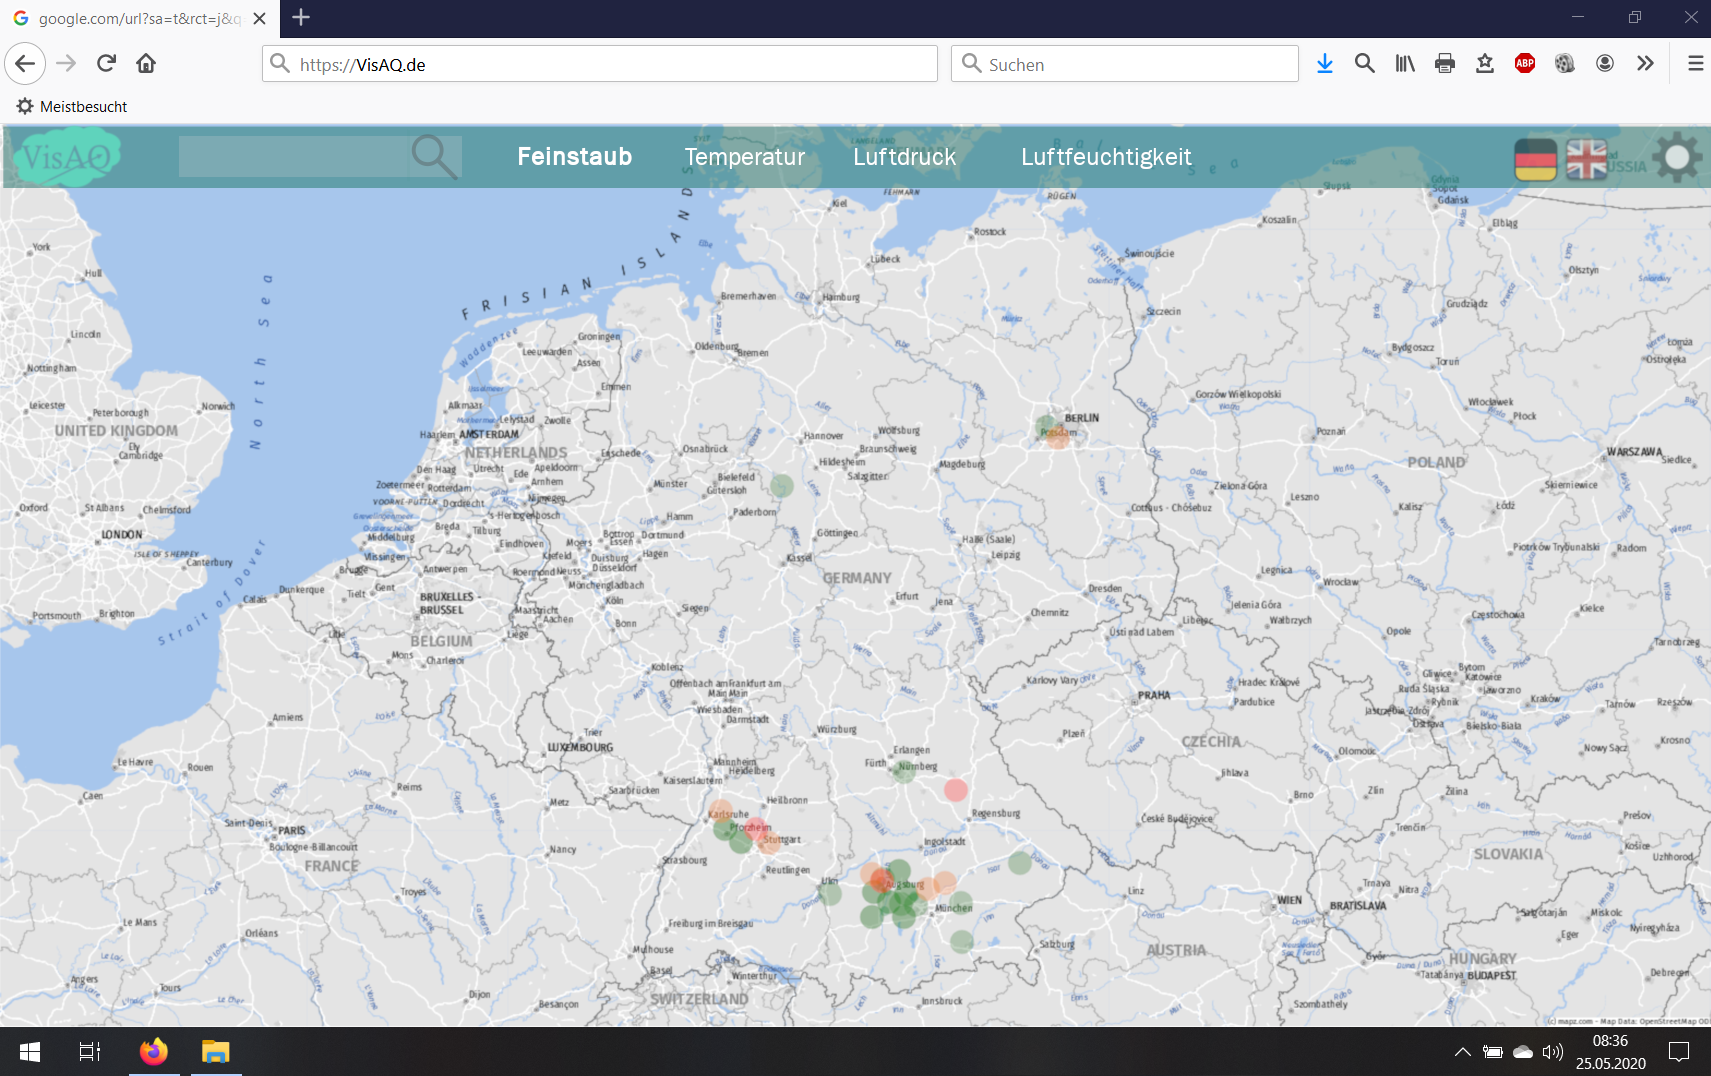
\includegraphics[width=0.9\textwidth]{Screenshots/Startseite}\captionof{figure}{Startseite} 
	
	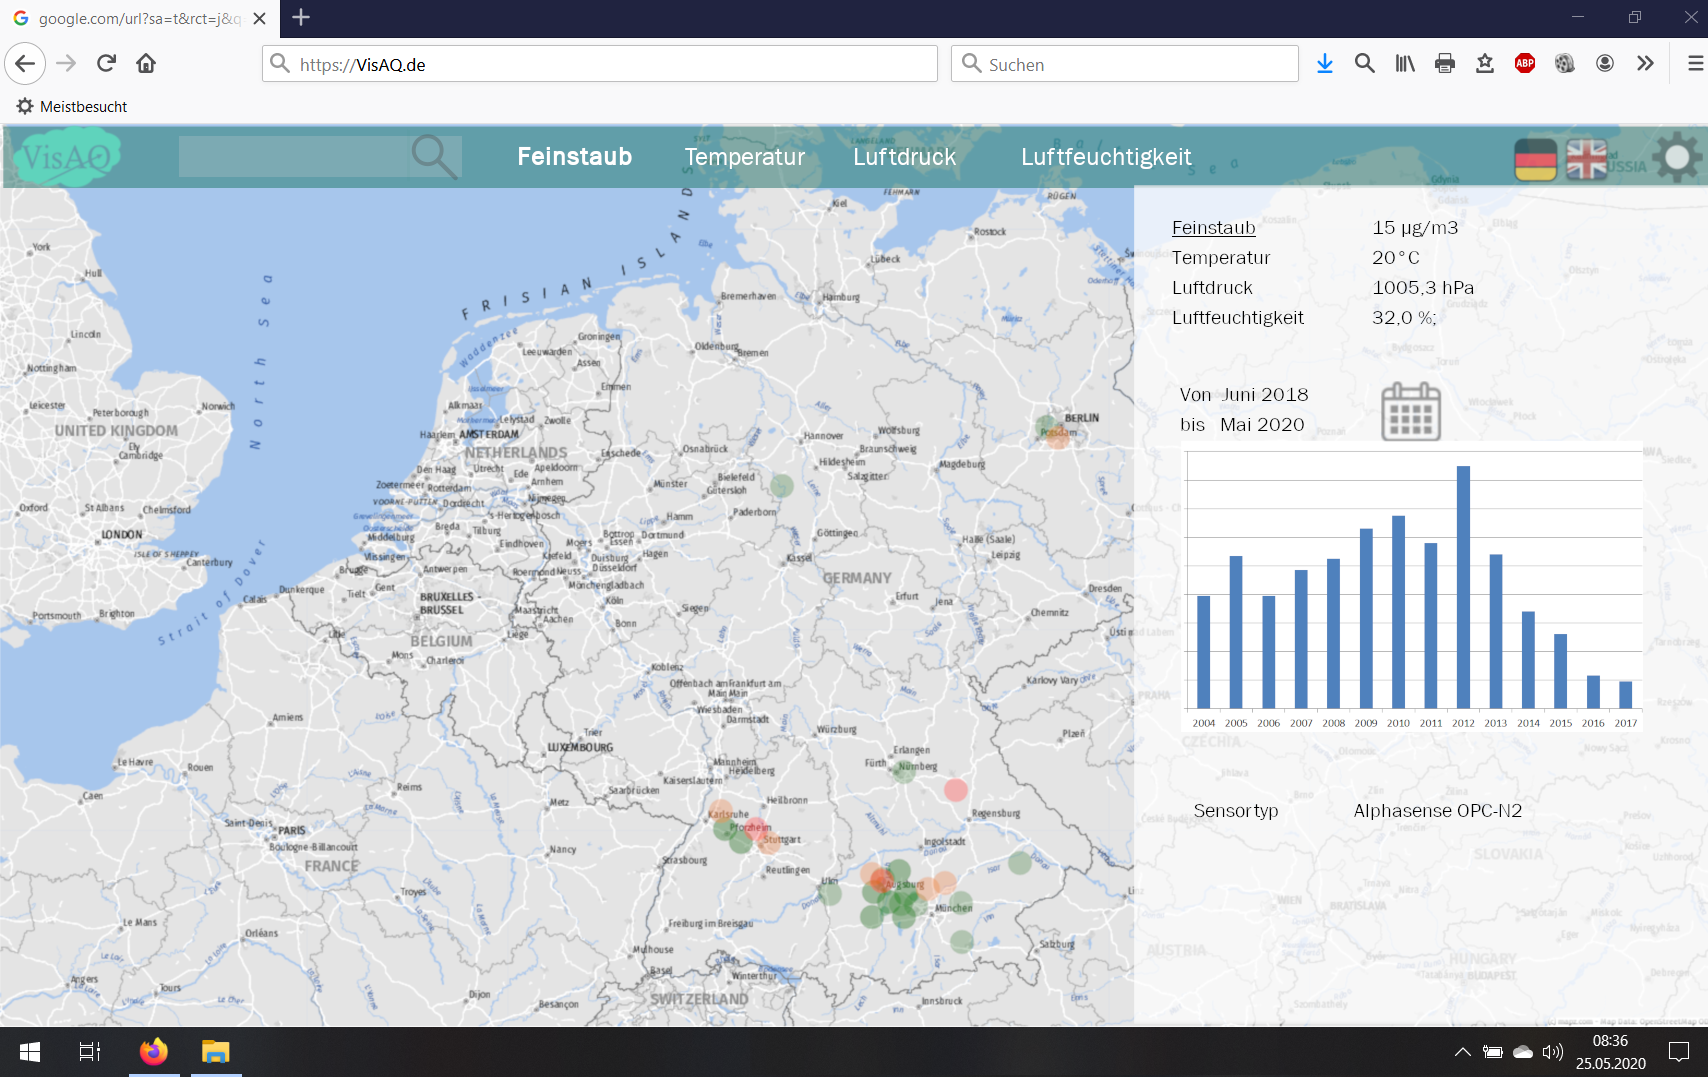
\includegraphics[width=0.9\textwidth]{Screenshots/Aktuelle-Daten}\captionof{figure}{Aktuelle Daten} 

	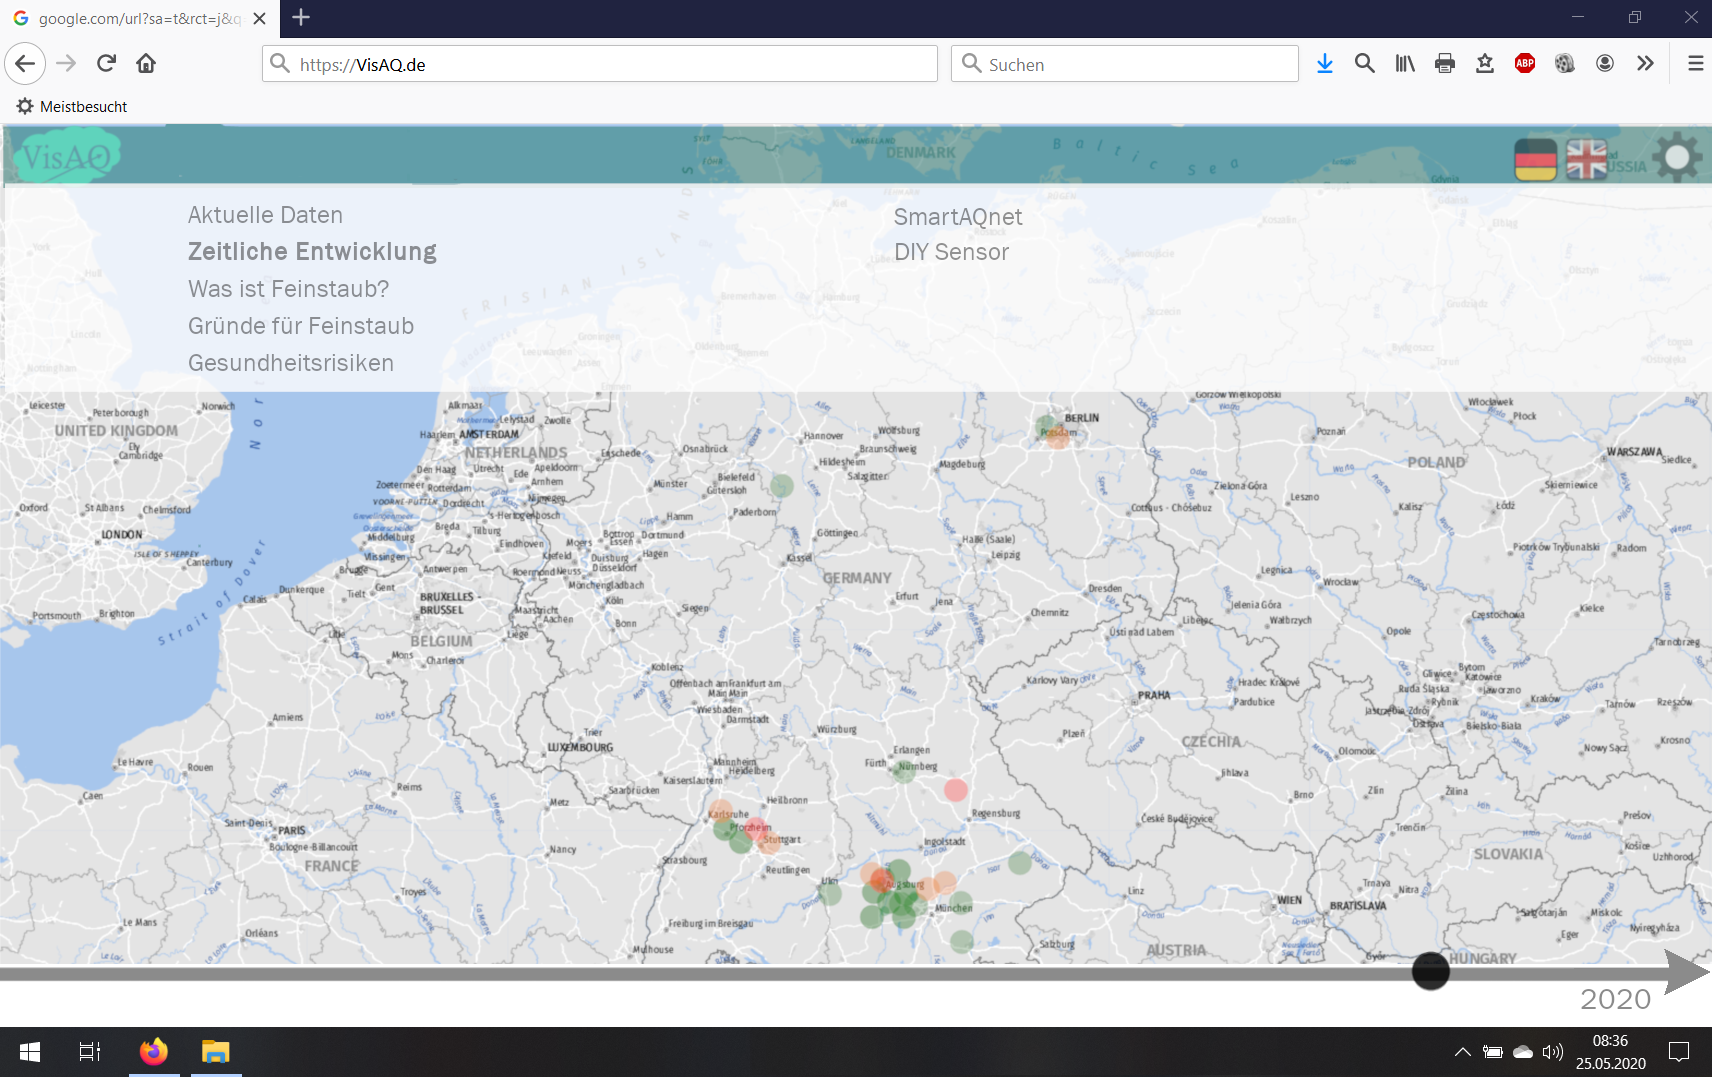
\includegraphics[width=0.9\textwidth]{Screenshots/Zeitliche-Entwicklung}\captionof{figure}{Zeitliche Entwicklung} 
	
	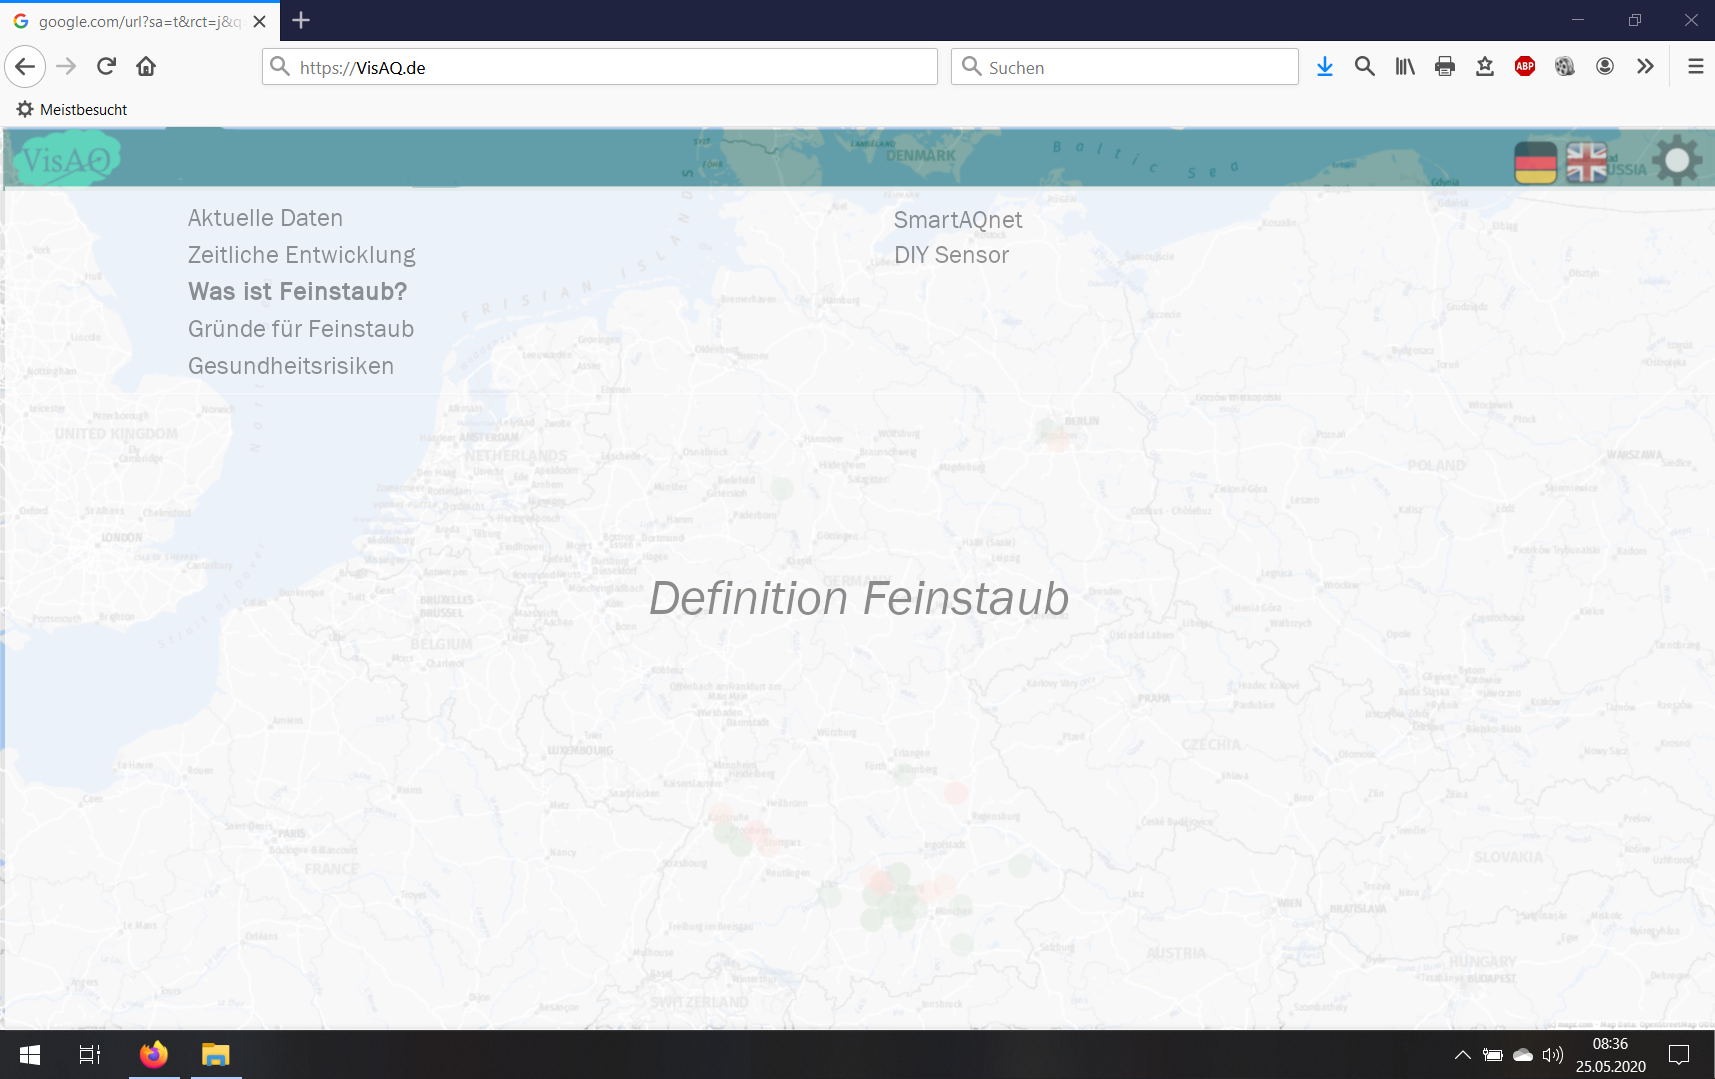
\includegraphics[width=0.9\textwidth]{Screenshots/Definition-von-Feinstaub}\captionof{figure}{Definition von Feinstaub} 
	
	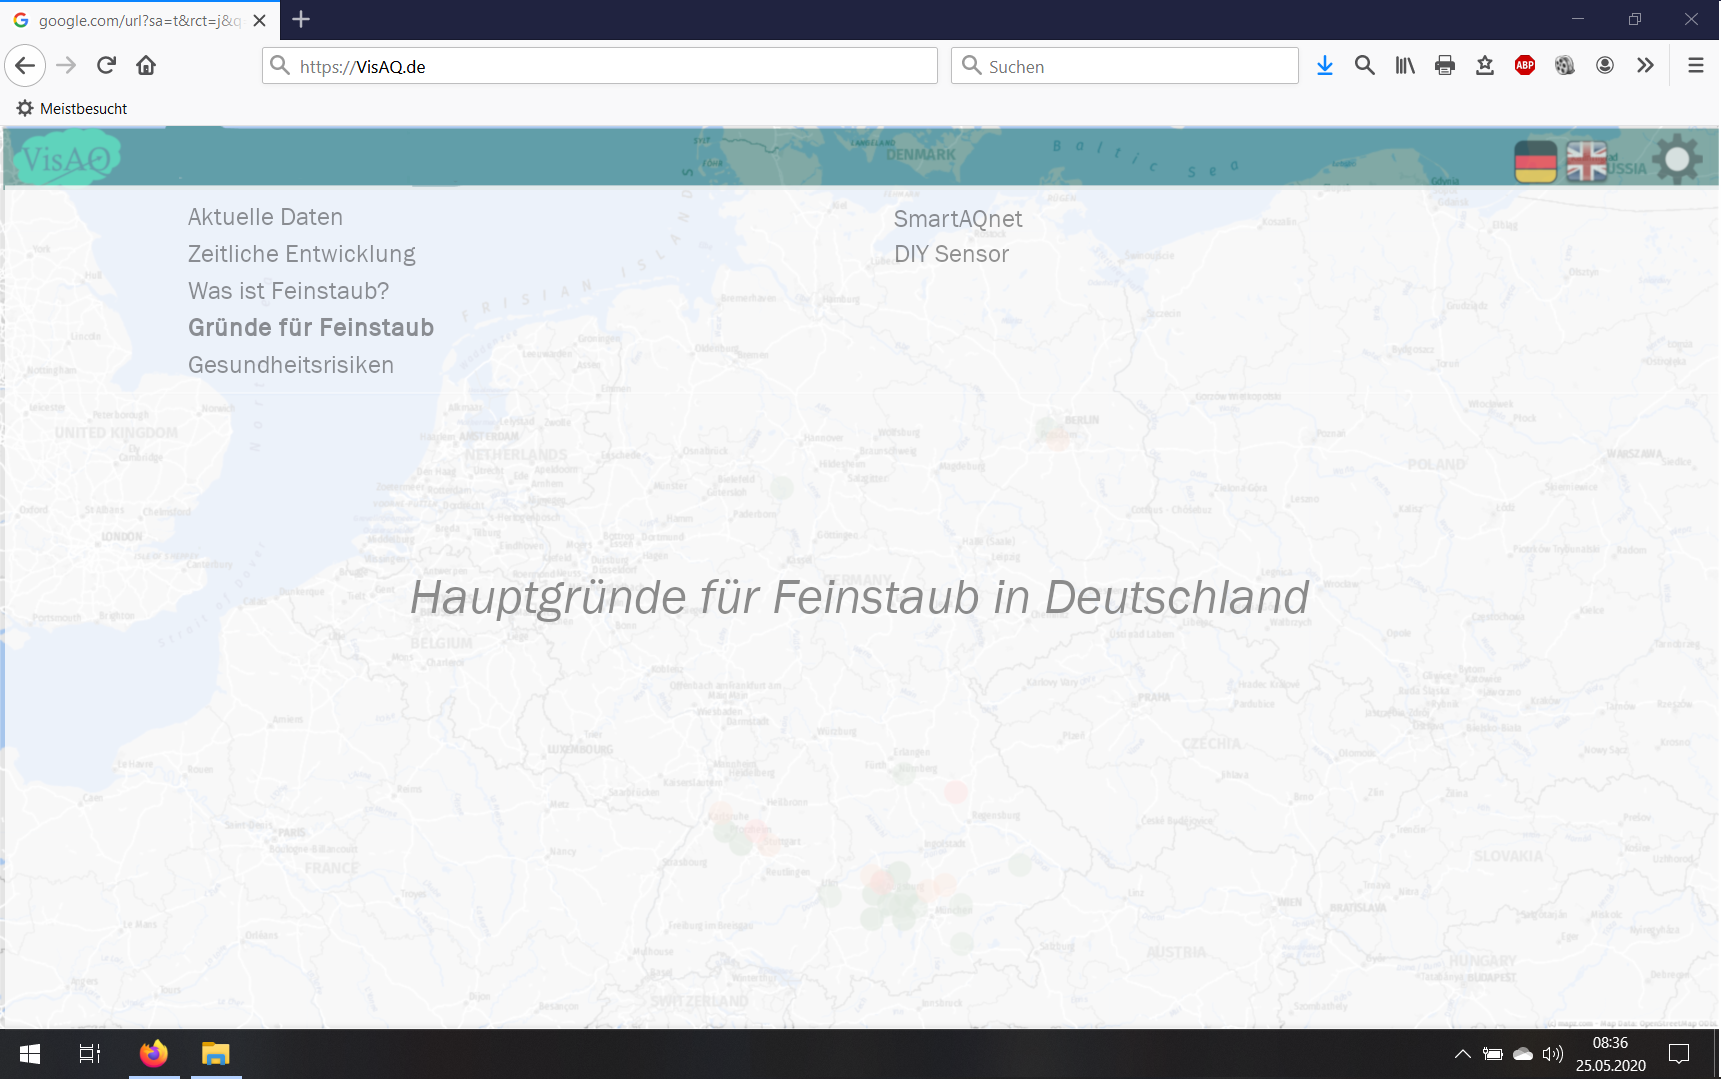
\includegraphics[width=0.9\textwidth]{Screenshots/Gruende-Feinstaub}\captionof{figure}{Hauptgründe für Feinstaub in Deutschland} 
	
	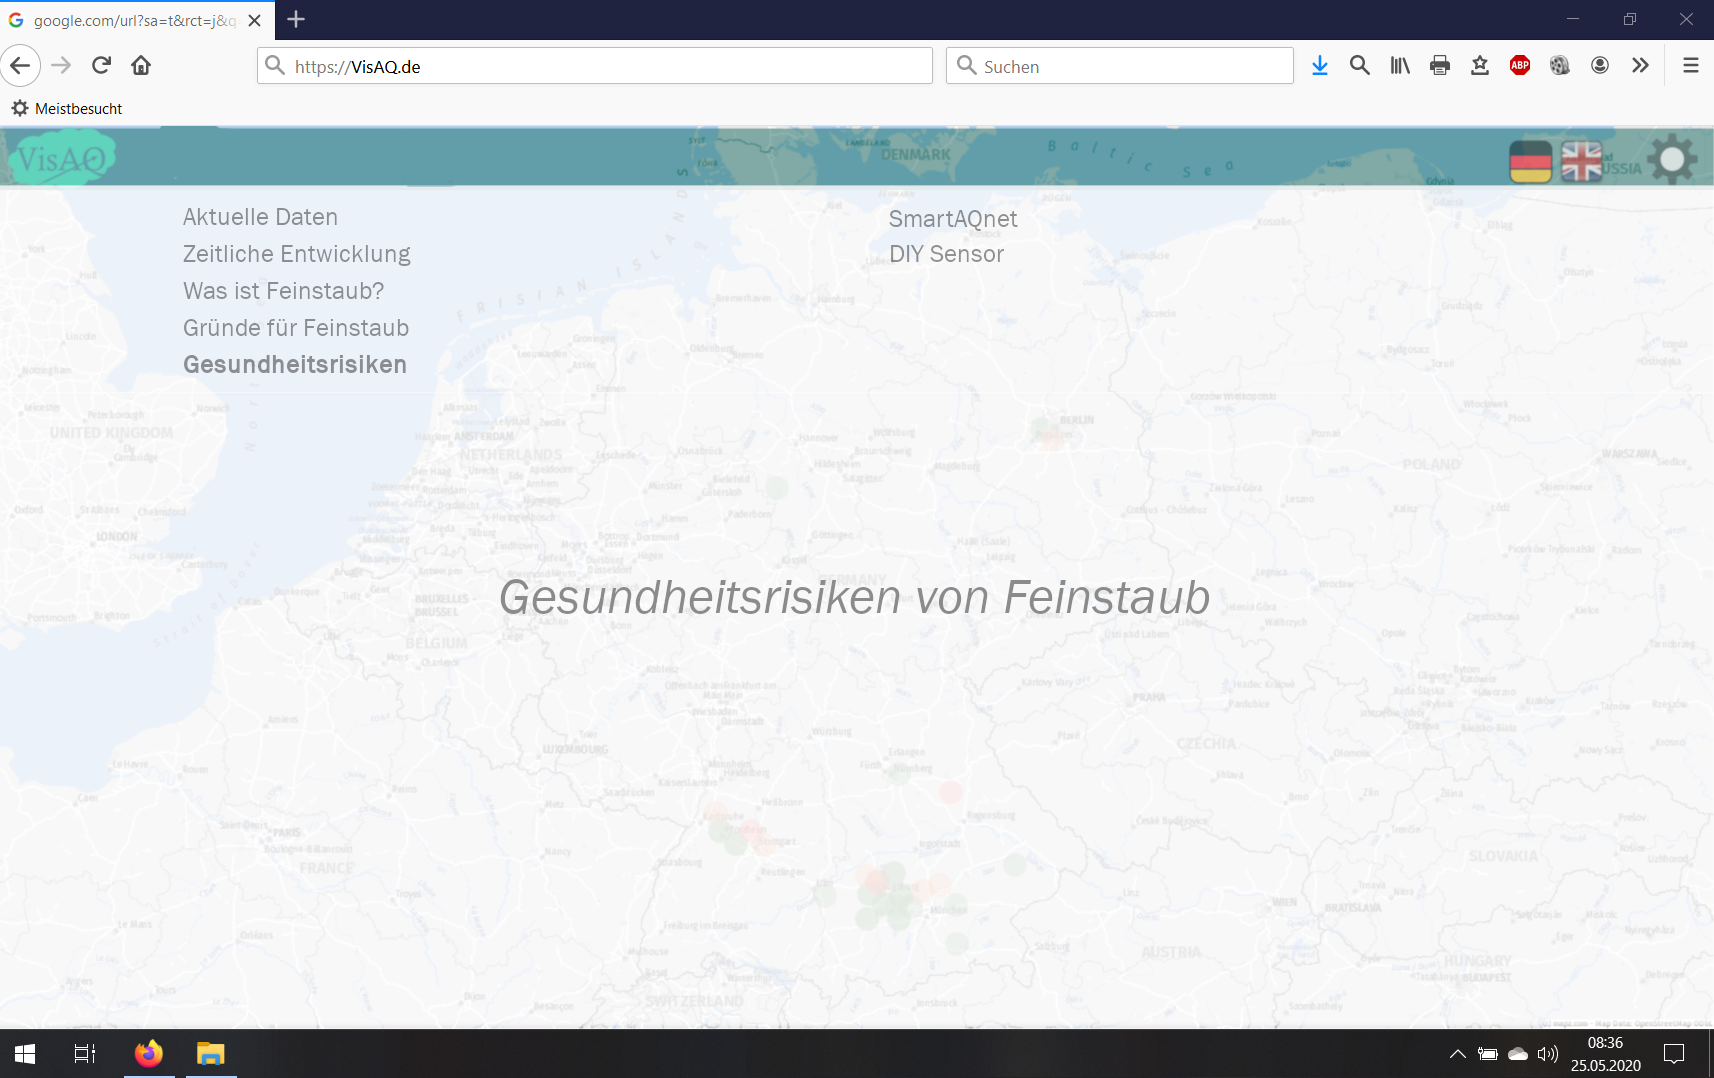
\includegraphics[width=0.9\textwidth]{Screenshots/Gesundheitsrisiken}\captionof{figure}{Gesundheitsrisiken von Feinstaub} 
	
	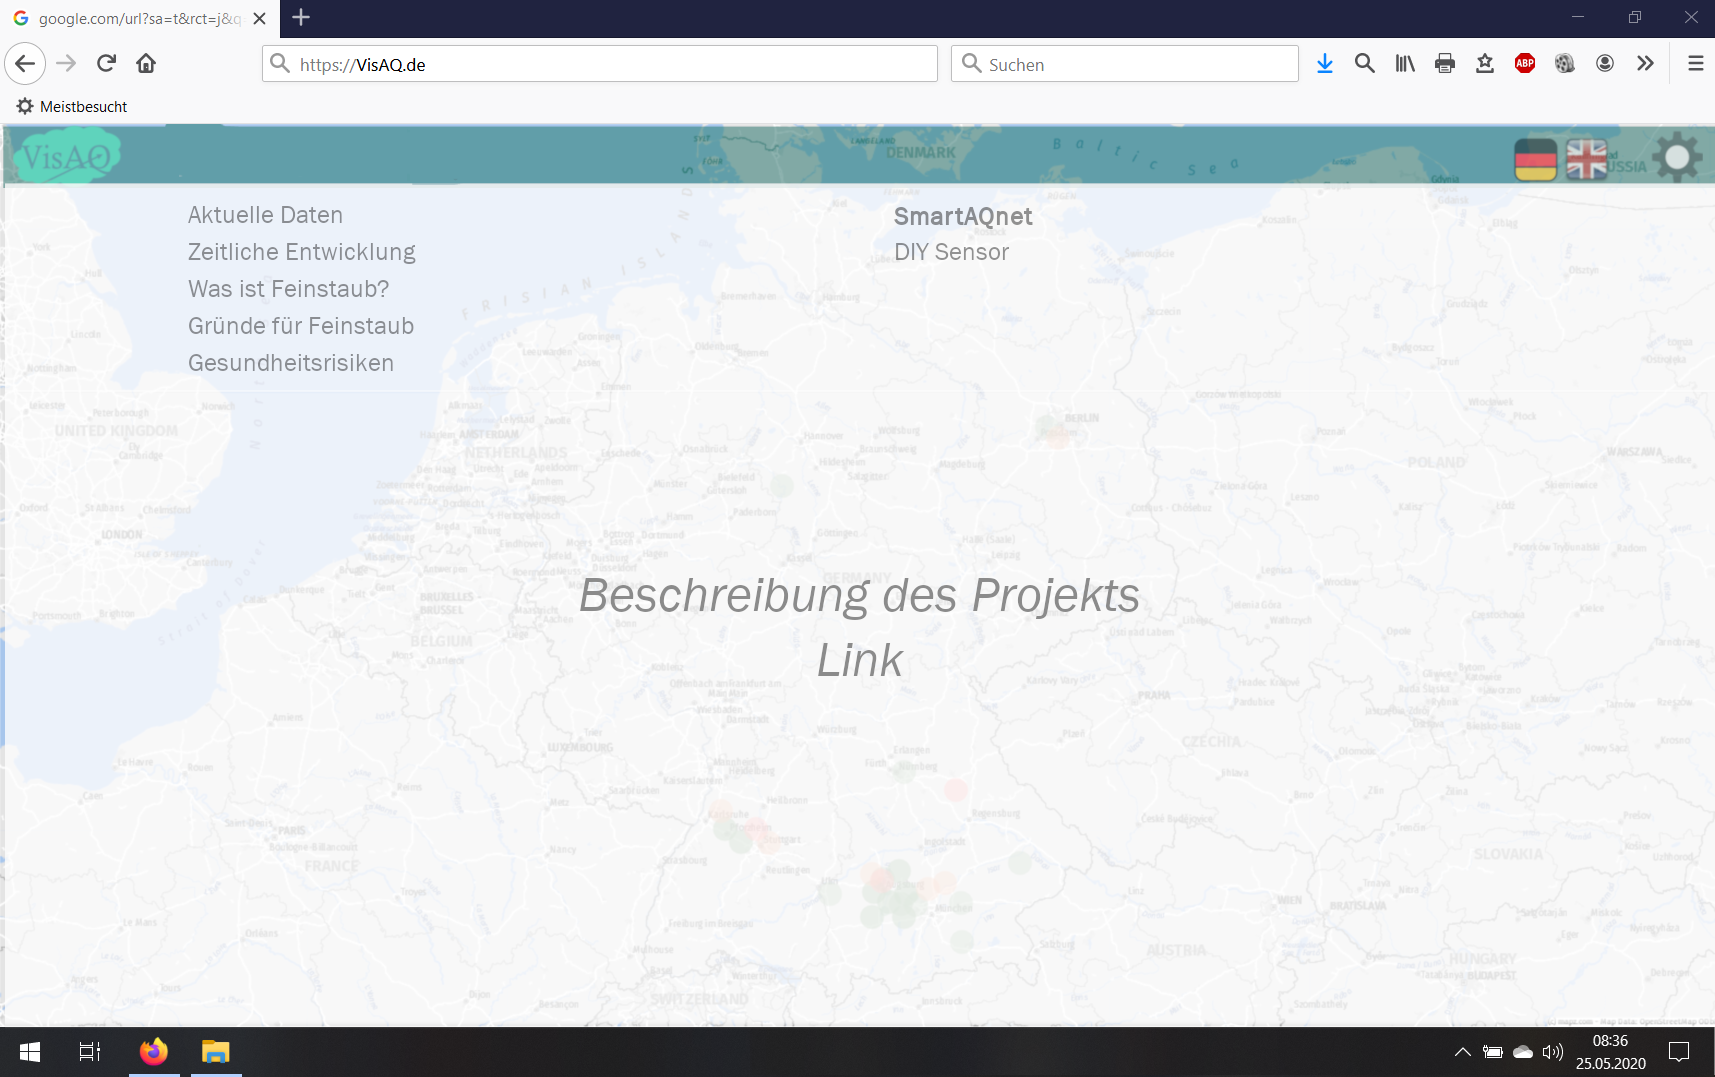
\includegraphics[width=0.9\textwidth]{Screenshots/SmartAQnet}\captionof{figure}{\glspl{SmartAQnet}} 
	
	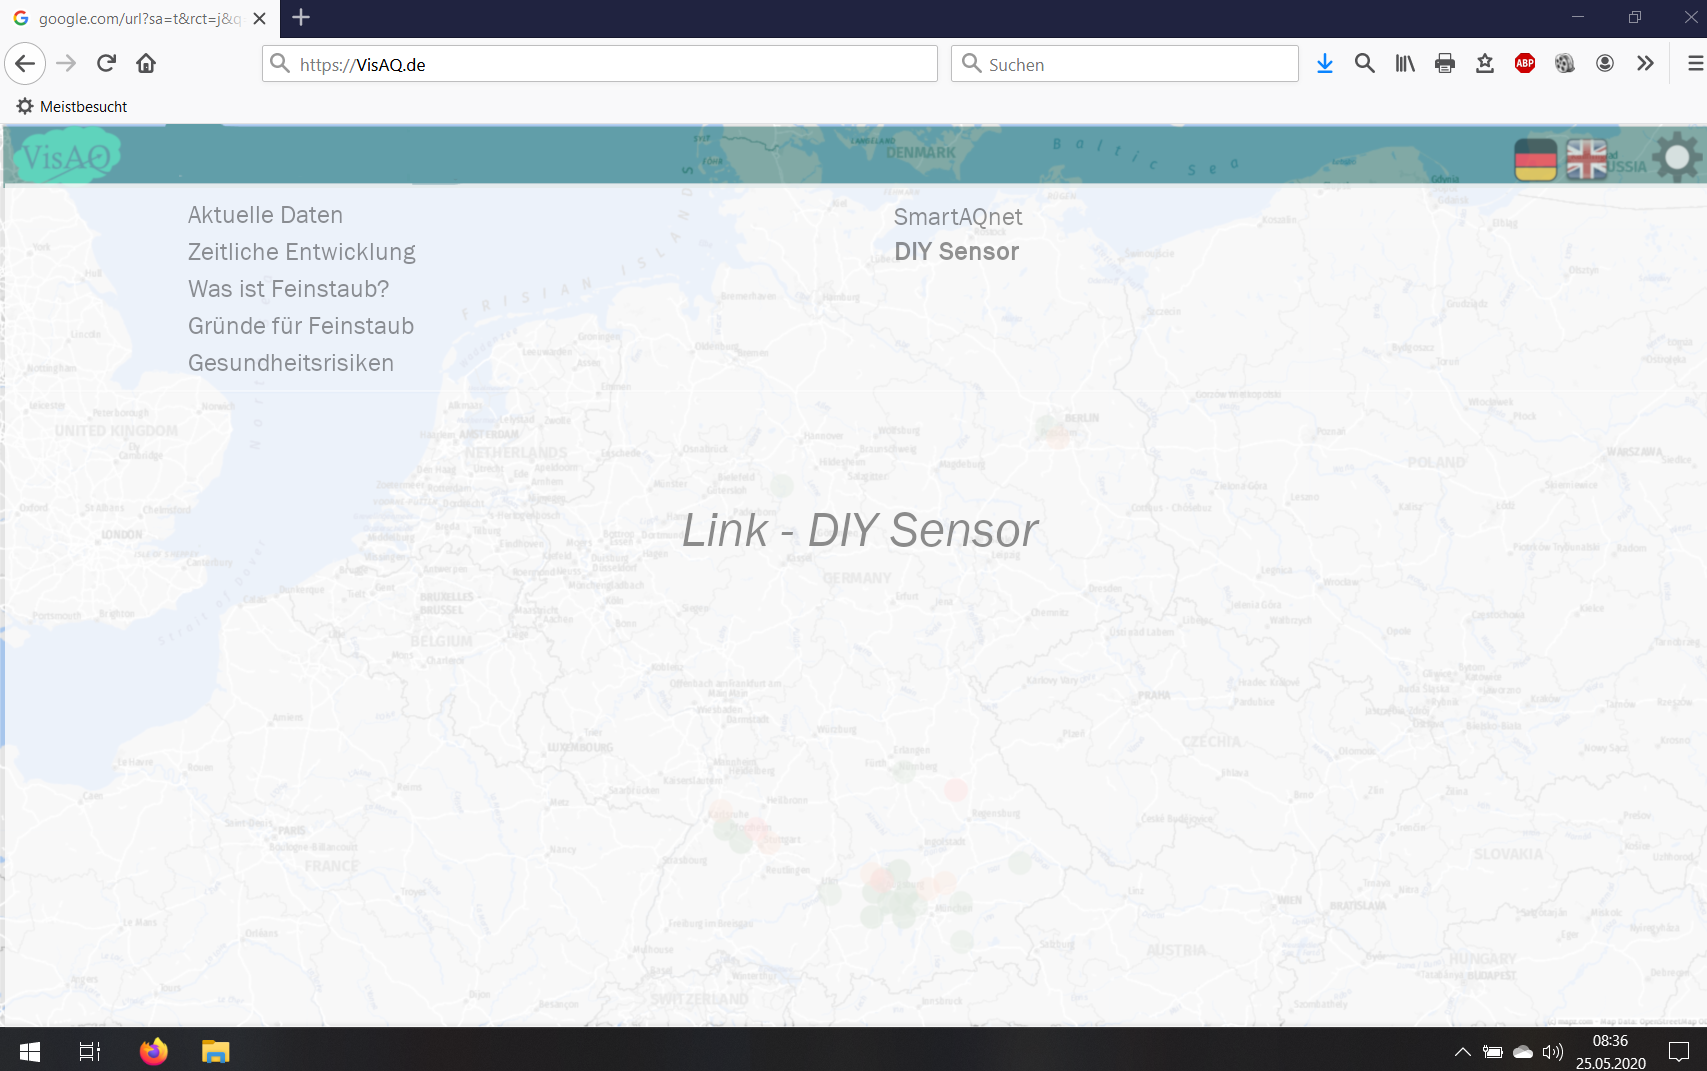
\includegraphics[width=0.9\textwidth]{Screenshots/DIY}\captionof{figure}{Verlinkung zu einer Bauanleitung für einen \glspl{DIY-Sensor}} 
\end{center}

\textbf{Anmerkung:}
Es gilt zu beachten, dass die beschriebene Benutzeroberfläche in \autoref{Struktur Frontend} und \autoref{Screenshots} nur eine erste Annäherung an das Endprodukt ist. In der endgültige Version sind eventuell Abweichungen in der Darstellung der Daten möglich, jedoch ist die hier gegebene Struktur maßgeblich.
